\documentclass{beamer}

\input{settings.tex}


\usepackage[T2A]{fontenc}
\usepackage[utf8]{inputenc}
\usepackage[english,russian]{babel}
\title{Домен, Выпуклость}
\subtitle{\mycoursetitle, Лекция 4}
\author{Сергей Савин}
\centering
\date{\mydate}



\begin{document}
\maketitle


\begin{frame}{Содержание}
	
	\begin{itemize}
		\item Задачи с ограничениями-неравенствами
		\item Квадратичное программирование
		\item Область определения. Ограниченные и неограниченные области.
		\item Выпуклые области
		\item Выпуклая комбинация
		\item Опорная гиперплоскость
		\item Выпуклые функции
		\item Неравенство Йенсена
		\item Надграфик (эпиграф)
	\end{itemize}
	
\end{frame}

\begin{frame}{Задачи с ограничениями-неравенствами}
	\begin{flushleft}
		
		Задача 1.
		%
		\begin{equation}
			\begin{aligned}
				& \underset{\mathbf{x}}{\text{minimize}}
				& & || \mathbf{D}\mathbf{x} + \mathbf{f} ||, \\
				& \text{subject to}
				& & \mathbf{x} \leq \mathbf{b}.
			\end{aligned}
		\end{equation}
		
		Задача 2.
		%
		\begin{equation}
			\begin{aligned}
				& \underset{\mathbf{x}}{\text{minimize}}
				& & || \mathbf{x} ||, \\
				& \text{subject to}
				& & \mathbf{A}\mathbf{x} \leq \mathbf{b}.
			\end{aligned}
		\end{equation}
		
		Задача 3.
		%
		\begin{equation}
			\begin{aligned}
				& \underset{\mathbf{x}}{\text{minimize}}
				& & || \mathbf{D}\mathbf{x} + \mathbf{f} ||, \\
				& \text{subject to}
				& & \begin{cases}
					\mathbf{A}\mathbf{x} \leq \mathbf{b}, \\
					\mathbf{C}\mathbf{x} = \mathbf{d}.
				\end{cases}
			\end{aligned}
		\end{equation}
		
	\end{flushleft}
\end{frame}

\begin{frame}{Квадратичное программирование}
	\begin{flushleft}
		
		Упомянутые задачи могут быть описаны вместе как задачи квадратичного программирования. Название обусловлено тем, что целевая функция является квадратичной (или эквивалентной). Допускается наличие линейных ограничений-равенств и ограничений-неравенств.
		
		\bigskip
		
		Общая форма задачи квадратичного программирования приведена ниже:
		
		%
		\begin{equation}
			\begin{aligned}
				& \underset{\mathbf{x}}{\text{minimize}}
				& & \mathbf{x}^\top \mathbf{H} \mathbf{x} + \mathbf{f}^\top\mathbf{x}, \\
				& \text{subject to}
				& & \begin{cases}
					\mathbf{A}\mathbf{x} \leq \mathbf{b}, \\
					\mathbf{C}\mathbf{x} = \mathbf{d}.
				\end{cases}
			\end{aligned}
		\end{equation}
		
		где $\mathbf{H}$ положительно определена, а $\mathbf{A}\mathbf{x} \leq \mathbf{b}$ описывает \emph{выпуклую область}.
		
	\end{flushleft}
\end{frame}

\begin{frame}
	\centerline{\huge Область определения (домен)}
	
	\bigskip
	
	\centerline{\huge Выпуклость}
\end{frame}


\begin{frame}{Область определения}
	\begin{flushleft}
		
		Задача 1. Найти минимум функции $f = x^2 + 2y^2$, если $x \in \mathbb{R}$ и $y \in \mathbb{R}$. \textcolor{white}{Решение: $x = 0$, $y = 0$.}
		
		\bigskip
		
		Задача 2. Найти минимум функции $f = x^2 + 2y^2$, если $x \in [1 ; 2]$ и $y \in [2 ; 5]$. \textcolor{white}{Решение: $x = 1$, $y = 2$.}
		
		\bigskip
		
		Заметим, что решения задач 1 и 2 различаются, и это связано исключительно с различием в допустимых значениях, которые могут принимать \emph{переменные решения} $x$ и $y$.
		
		\begin{block}{Определение 1}
			Пространство всех допустимых значений, которые могут принимать переменные решения, называется \emph{областью определения} задачи оптимизации.
		\end{block}
		
	\end{flushleft}
\end{frame}

\begin{frame}{Ограниченные и неограниченные области, 1}
	\begin{flushleft}
		
		Задача 3. Найти минимум функции $f = -x^2$, если $x \in [-3 ; 2]$. \textcolor{white}{Решение: $x = -3$.}
		
		\bigskip
		
		Задача 4. Найти минимум функции $f = -x^2$, если $x \in \mathbb{R}$. \textcolor{white}{Задача не имеет решения.}
		
		\bigskip
		
		Задача 5. Найти минимум функции $f = -x^2$, если $x \in (-\infty ; 2]$. \textcolor{white}{Задача не имеет решения.}
		
		\bigskip
		
		Основное различие между областями определения задач 2, 3 и задачами 1, 4, 5 заключается в том, что последние являются \emph{неограниченными} (т.е. можно построить последовательность значений в области, которая стремится к бесконечности).
		
		\bigskip
		
		Мы видим, что в случае задач 3-5 ограниченная область позволяет задаче иметь решение \textcolor{mygray}{(непрерывная функция на компактном множестве (замкнутом + ограниченном) достигает своего минимума)}.
		
	\end{flushleft}
\end{frame}

\begin{frame}{Ограниченные и неограниченные области, 2}
	\begin{flushleft}
		
		Задача 6. Найти максимум функции $f = x^2$, если $1 \leq x < 2$. \textcolor{white}{Не имеет решения.}
		
		\bigskip
		
		Задача 7. Найти минимум функции $f = x^2$, если $1 \leq x < 2$. \textcolor{white}{Решение: $x = 1$.}
		
		\bigskip
		
		В данном случае одна из \emph{границ} области не была включена (область не является \emph{замкнутой}). Именно поэтому задача 6 не имеет решения, в то время как задача 7 решение имеет.
		
		\bigskip
		
		Для задачи 6 мы можем выбрать значение сколь угодно близкое к $x = 2$, приближаясь к нему слева, но для любого такого значения всегда найдутся другие значения переменной решения, еще более близкие к $x = 2$ и, следовательно, дающие большие значения $f$.
		
	\end{flushleft}
\end{frame}

\begin{frame}{Выпуклые области}
	\begin{flushleft}
		
		\begin{block}{Определение 2}
			Область называется \emph{выпуклой}, если для любых двух точек из области отрезок, их соединяющий, также целиком принадлежит области.
		\end{block}
		
		\bigskip
		
		\begin{figure}
			\centering
			\begin{minipage}{.3\textwidth}
				\centering
				
				\textit{
					\begin{tikzpicture}[x=0.75pt,y=0.75pt,yscale=-1,xscale=1]
						\draw [fill={rgb, 255:red, 255; green, 160; blue, 160 } ,fill opacity=1 ] (148,55) -- (188,62.5) -- (211,107.5) -- (175,170.5) -- (94,158.5) -- (98,85) -- cycle ;
				\end{tikzpicture}}
				
				\captionof{figure}{Выпуклая область}
			\end{minipage}%
			\begin{minipage}{.7\textwidth}
				\centering
				
				\begin{tikzpicture}[x=0.75pt,y=0.75pt,yscale=-1,xscale=1]
					\draw [fill={rgb, 255:red, 255; green, 160; blue, 160 } ,fill opacity=1 ] (525,68.5) -- (525,112.5) -- (452,97.5) -- (435,120.5) -- (533,188.5) -- (488,204.5) -- (411,187.5) -- (404,72.5) -- cycle ;
					\draw [color={rgb, 255:red, 208; green, 2; blue, 27 } ,draw opacity=1, line width=1.75pt ] (501,88.5) -- (486.03,126.12) -- (464,181.5) ;
				\end{tikzpicture}
				
				\captionof{figure}{Невыпуклая область}
			\end{minipage}
		\end{figure}
		
	\end{flushleft}
\end{frame}




\begin{frame}{Выпуклая комбинация, 1}
	\begin{flushleft}
		
		В доказательствах удобно помнить, что для любых двух точек $\mathbf{x}_1$ и $\mathbf{x}_2$ все точки отрезка, их соединяющего, задаются как $\mathbf{x}_l = \alpha \mathbf{x}_1 + (1 - \alpha) \mathbf{x}_2$, где $\alpha \in [0 \; 1]$. Это называется \emph{выпуклой комбинацией}.
		
		\bigskip
		
		Можно представить переменную $\alpha$ как ползунок — перемещая $\alpha$ от 0 до 1, мы перемещаем $\bo{x}_l$ от $\bo{x}_2$ до $\bo{x}_1$.
		
		\bigskip
		
		Отрезок между точками $\bo{x}_1$ и $\bo{x}_2$ является \emph{выпуклой оболочкой} точек $\bo{x}_1$ и $\bo{x}_2$. Его можно определить как:
		
		\begin{equation}
			\mathcal{L} = \{ \bo{x}: \ \bo{x}=\alpha \bo{x}_1 + (1 - \alpha) \bo{x}_2, \ \alpha \in [0 \; 1] \}
		\end{equation}
		
	\end{flushleft}
\end{frame}

\begin{frame}{Выпуклая комбинация, 2}
	\begin{flushleft}
		
		Эквивалентно, выпуклая комбинация (отрезок) двух точек $\bo{x}_1$ и $\bo{x}_2$ задается как:
		
		\begin{equation}
			\mathcal{L} = \{ \bo{x}: \ \beta_1 \bo{x}_1 + \beta_2 \bo{x}_2, \ \beta_1+\beta_2 = 1, \ \beta_{1, 2} \in [0 \; 1] \}
		\end{equation}
		
		Чтобы показать эквивалентность, заметим, что $\beta_1 = 1 - \beta_2$. Определяя $\alpha = \beta_1$, получаем $\beta_2 = 1 - \alpha$, где $\alpha \in [0 \; 1]$, что и доказывает эквивалентность.
		
	\end{flushleft}
\end{frame}

\begin{frame}{Примеры выпуклых областей, 1}
	\begin{flushleft}
		
		$\mathbf{x} \in \mathcal{X}$, $\mathcal{X} = \mathbb{R}^n$ выпукла.
		
		\bigskip
		
		$\mathbf{x} \in \mathcal{X}$, $\mathcal{X} = \{ \mathbf{x} \in \mathbb{R}^n: \ \mathbf{x} \leq \mathbf{h} \}$ выпукла.
		
		\bigskip
		
		Доказательство: Заметим, что $\alpha \mathbf{x}_1 \leq \alpha \mathbf{h}$ и $(1 - \alpha) \mathbf{x}_2 \leq (1 - \alpha) \mathbf{h}$, следовательно, $\alpha \mathbf{x}_1 + (1 - \alpha) \mathbf{x}_2 \leq 
		\alpha \mathbf{h} + (1 - \alpha) \mathbf{h} = \mathbf{h}$. \qedsymbol
		
		\bigskip
		
		$\mathbf{x} \in \mathcal{X}$, $\mathcal{X} = \{ \mathbf{x} \in \mathbb{R}^2: \ x_1^2+x_2^2 \leq h^2 \}$ выпукла.
		
		\bigskip
		
		Доказательство: Пусть $\mathbf{x}_1, \mathbf{x}_2 \in \mathcal{X}$, так что 
		$\|\mathbf{x}_1\| \le h$ и $\|\mathbf{x}_2\| \le h$. Тогда для любого $\alpha \in [0,1]$:
		\[  
		\|\alpha \mathbf{x}_1 + 
		\underset{\textcolor{mygray}{\text{неравенство треугольника}}}{(1-\alpha)\mathbf{x}_2\| \le \alpha \|\mathbf{x}_1\| }
		+ (1-\alpha)\|\mathbf{x}_2\|
		\le \alpha h + (1-\alpha)h = h. \ \ \  \qedsymbol
		\] 
		
	\end{flushleft}
\end{frame}

\begin{frame}{Примеры выпуклых областей, 2}
	\begin{flushleft}
		
		$\mathbf{x} \in \mathcal{X}$, $\mathcal{X} = \{ \mathbf{x} \in \mathbb{R}^n: \ \mathbf{x}^\top \mathbf{H} \mathbf{x} \leq 1 \}$, где $\mathbf{H} \succ 0$ — положительно определенная симметричная матрица, выпукла.
		
		\bigskip
		
		Для любой положительно определенной симметричной $\mathbf{H}$ верно, что $\mathbf{H} = \mathbf{D}^\top\mathbf{D}$, где $\mathbf{D} = \sqrt{\mathbf{H}}$ называется квадратным корнем матрицы и имеет полный ранг.
		
		\bigskip
		
		При этом $\mathbf{x}^\top \mathbf{H} \mathbf{x} \leq 1$ превращается в $\mathbf{x}^\top \mathbf{D}^\top\mathbf{D} \mathbf{x} \leq 1$. Определяя $\mathbf{y} = \mathbf{D} \mathbf{x}$, получаем $\mathcal{X} = \{ \mathbf{D}^{-1}\mathbf{y}: \ \mathbf{y}^\top \mathbf{y} \leq 1 \}$. Это линейно деформированный шар, и, как таковой, он также выпукл. \textbf{Линейные (аффинные) преобразования сохраняют выпуклость.}
		
	\end{flushleft}
\end{frame}



\begin{frame}{Примеры невыпуклых областей}
	\begin{flushleft}
		
		Докажите следующие утверждения:
		
		$x \in \mathcal{X}$, $\mathcal{X} = [-1 ; 2] \cup [3 ; 7]$ не является выпуклой.
		
		\bigskip
		
		$\mathbf{x} \in \mathcal{X}$, $\mathcal{X} = { \mathbf{x} \in \mathbb{R}^2: \ x_1^2+x_2^2 \geq h^2 }$ не является выпуклой.
		
		\bigskip
		
		$\mathbf{x} \in \mathcal{X}$, $\mathcal{X} = { \mathbf{x} \in \mathbb{R}^n: \ \mathbf{x}^\top \mathbf{H} \mathbf{x} \geq 1 }$, где $\mathbf{H} \succ 0$, не является выпуклой.
		
		\bigskip
		
		Для этих доказательств достаточно единственного контрпримера, чтобы показать, что определяющее свойство выпуклых областей не выполняется.
		
	\end{flushleft}
\end{frame}

\begin{frame}{Опорная гиперплоскость}
	\begin{flushleft}
		
		Для выпуклого множества $\mathcal C$ и точки $\bo{x}_0$ на его границе, если неравенство $\bo{a}\T \bo{x} \leq \bo{a}\T \bo{x}_0$ выполняется для $\forall \bo{x} \in \mathcal C$, то $\bo{a}\T \bo{x} = \bo{a}\T \bo{x}_0$ является \emph{опорной гиперплоскостью}.
		
		\begin{figure}
			\centering
			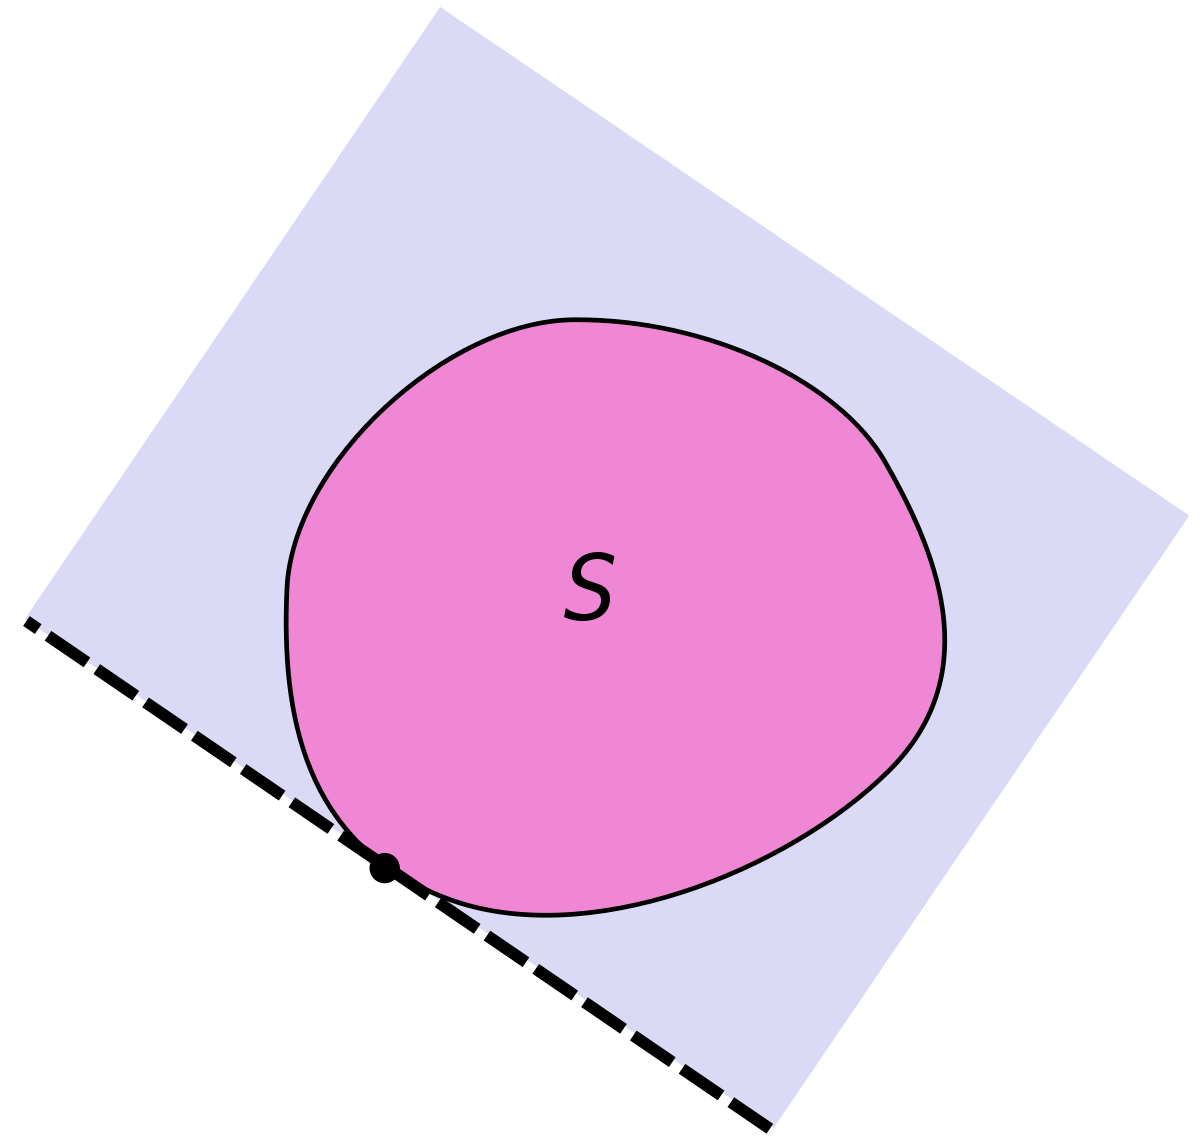
\includegraphics[width=0.5\linewidth]{Supporting_hyperplane}
			\caption{Опорная гиперплоскость}%(source: wikipedia)
			\label{fig:supportinghyperplane}
		\end{figure}
		
	\end{flushleft}
\end{frame}

\begin{frame}{Пример — инверсная динамика}
	\begin{flushleft}
		
		Рассмотрим динамическую систему:
		%
		\begin{equation}
			\bo{H} \bo{a} + \bo{C}\dot{\bo{q}} + \bo{g} = \bo{B}\bo{u}
		\end{equation}
		
		Для текущего состояния $\bo{q}$, $\dot{\bo{q}}$ найти такое $\bo{u}$, которое делает $\bo{a}$ наиболее близким к желаемому значению $\bo{a}_d$, \textcolor{mydarkred}{требуя, чтобы каждая компонента $\bo{u}$ по абсолютной величине не превышала порога $u_{max}$}.
		
		\bigskip
		
		\textbf{Решение}:
		%
		\begin{equation}
			\begin{aligned}
				& \underset{\bo{u}, \bo{a}}{\text{minimize}}
				& & (\bo{a}-\bo{a}_d)\T (\bo{a}-\bo{a}_d), \\
				& \text{subject to}
				& & \begin{cases}
					\bo{H} \bo{a} + \bo{C}\dot{\bo{q}} + \bo{g} = \bo{B}\bo{u} \\
					|u_i| \leq u_{max}, \ \forall i
				\end{cases}
			\end{aligned}
		\end{equation}
		
		Область, описываемая неравенствами $|u_i| \leq u_{max}$, является \textbf{выпуклой}.
		
	\end{flushleft}
\end{frame}

\begin{frame}{Пример — планирование положения}
	\begin{flushleft}
		
		Найти положение $\bo{r} = [x, \ y]\T$ робота, наиболее близкое к желаемому положению $\bo{r}_d= [x_d, \ y_d]\T$, но \textcolor{mydarkred}{находящееся не менее чем на 5 м от наземной станции и не более чем на 100 м от наземной станции.} Положение наземной станции — $\bo{r}_g= [x_g, \ y_g]\T$.
		
		\bigskip
		
		\textbf{Решение}:
		%
		\begin{equation}
			\begin{aligned}
				& \underset{x, y}{\text{minimize}}
				& & (x-x_d)^2 + (y-y_d)^2, \\
				& \text{subject to}
				& & \begin{cases}
					(x-x_g)^2 + (y-y_g)^2 \ge 5^2 \\
					(x-x_g)^2 + (y-y_g)^2 \le 100^2
				\end{cases}
			\end{aligned}
		\end{equation}
		
		Область, описываемая этими неравенствами, \textbf{не является выпуклой}.
		
	\end{flushleft}
\end{frame}

\begin{frame}
	\centerline{\huge Выпуклые функции}
\end{frame}



\begin{frame}{Выпуклые функции}
	\begin{flushleft}
		
		Функция называется выпуклой, если для любых двух точек на ее графике отрезок, их соединяющий, лежит выше графика.
		
		\begin{figure}
	\centering
	\begin{minipage}{.4\textwidth}
		\centering
		
		\begin{tikzpicture}[x=0.75pt,y=0.75pt,yscale=-1,xscale=1]
			\draw  [draw opacity=0, line width=1.0pt] (696.23,142.36) .. controls (681.43,167.71) and (649.5,185.54) .. (612.24,186.11) .. controls (573.51,186.7) and (539.97,168.5) .. (525.19,141.99) -- (611.08,111.08) -- cycle ; \draw   (696.23,142.36) .. controls (681.43,167.71) and (649.5,185.54) .. (612.24,186.11) .. controls (573.51,186.7) and (539.97,168.5) .. (525.19,141.99) ;
			\draw [color={rgb, 255:red, 208; green, 2; blue, 27 }  ,draw opacity=1, line width=1.75pt]   (680,161.5) -- (560,173.5) ;
			
			\draw [color={rgb, 255:red, 208; green, 2; blue, 27 }  ,draw opacity=1 ]   (680,161.5) -- (560,173.5) ;
			%Shape: Circle [id:dp3160827101885906] 
			\draw  [fill={rgb, 255:red, 0; green, 0; blue, 0 }  ,fill opacity=1 ] (554.5,173.5) .. controls (554.5,170.46) and (556.96,168) .. (560,168) .. controls (563.04,168) and (565.5,170.46) .. (565.5,173.5) .. controls (565.5,176.54) and (563.04,179) .. (560,179) .. controls (556.96,179) and (554.5,176.54) .. (554.5,173.5) -- cycle ;
			%Shape: Circle [id:dp16415395117171228] 
			\draw  [fill={rgb, 255:red, 0; green, 0; blue, 0 }  ,fill opacity=1 ] (674.5,161.5) .. controls (674.5,158.46) and (676.96,156) .. (680,156) .. controls (683.04,156) and (685.5,158.46) .. (685.5,161.5) .. controls (685.5,164.54) and (683.04,167) .. (680,167) .. controls (676.96,167) and (674.5,164.54) .. (674.5,161.5) -- cycle ;
			
			\draw (560,185) node [anchor=north west][inner sep=0.75pt]   [align=left] {$\mathbf{x_1}$};
			\draw (675,170) node [anchor=north west][inner sep=0.75pt]   [align=left] {$\mathbf{x_2}$};
		\end{tikzpicture}
		\captionof{figure}{Convex function}
	\end{minipage}%
	\begin{minipage}{.7\textwidth}
		\centering
		
		\begin{tikzpicture}[x=0.75pt,y=0.75pt,yscale=-1,xscale=1]
			%uncomment if require: \path (0,300); %set diagram left start at 0, and has height of 300
			
			%Straight Lines [id:da6875192047258083] 
			\draw [color={rgb, 255:red, 208; green, 2; blue, 27 }  ,draw opacity=1, line width=1.75pt]   (564.6,165.5) -- (444.6,177.5) ;
			%Shape: Circle [id:dp14324656781298462] 
			\draw  [fill={rgb, 255:red, 0; green, 0; blue, 0 }  ,fill opacity=1 ] (439.1,177.5) .. controls (439.1,174.46) and (441.56,172) .. (444.6,172) .. controls (447.64,172) and (450.1,174.46) .. (450.1,177.5) .. controls (450.1,180.54) and (447.64,183) .. (444.6,183) .. controls (441.56,183) and (439.1,180.54) .. (439.1,177.5) -- cycle ;
			%Shape: Circle [id:dp2582069443071713] 
			\draw  [fill={rgb, 255:red, 0; green, 0; blue, 0 }  ,fill opacity=1 ] (559.1,165.5) .. controls (559.1,162.46) and (561.56,160) .. (564.6,160) .. controls (567.64,160) and (570.1,162.46) .. (570.1,165.5) .. controls (570.1,168.54) and (567.64,171) .. (564.6,171) .. controls (561.56,171) and (559.1,168.54) .. (559.1,165.5) -- cycle ;
			%Curve Lines [id:da47039197462224447] 
			\draw    (498.2,186.8) .. controls (512.6,148) and (529.4,88) .. (547.4,128) ;
			%Curve Lines [id:da13389450894014865] 
			\draw    (399,161.2) .. controls (439,131.2) and (470.6,244.8) .. (498.2,186.8) ;
			%Curve Lines [id:da2313253314744761] 
			\draw    (547.4,128) .. controls (563.8,173.6) and (577.4,192) .. (617.4,162) ;
			
			\draw (440,190) node [anchor=north west][inner sep=0.75pt]   [align=left] {$\mathbf{x_1}$};
			\draw (560,180) node [anchor=north west][inner sep=0.75pt]   [align=left] {$\mathbf{x_2}$};
		\end{tikzpicture}
		\captionof{figure}{Non-convex function}
	\end{minipage}
\end{figure}
		
	\end{flushleft}
\end{frame}

\begin{frame}{Неравенство Йенсена}
	\begin{flushleft}
		
		\begin{block}{Определение 3}
			Функция $f(\mathbf{x})$, определенная на области $\mathcal{D}$, для которой выполняется $\forall \mathbf{x}_1, \mathbf{x}_2 \in \mathcal{D}$, $f(\alpha \mathbf{x}_1 + (1 - \alpha) \mathbf{x}_2) \leq \alpha f(\mathbf{x}_1) + (1 - \alpha) f(\mathbf{x}_2)$, называется \emph{выпуклой функцией}.
		\end{block}
		
		\bigskip
		
		Это \emph{неравенство Йенсена}. Его можно эквивалентно переписать как:
		%
		\begin{align}
			\begin{cases}
				f(\alpha_1 \mathbf{x}_1 + \alpha_2 \mathbf{x}_2) \leq \alpha_1 f(\mathbf{x}_1) + \alpha_2 f(\mathbf{x}_2)
				\\
				\alpha_1 + \alpha_2 = 1
			\end{cases}
		\end{align}
		
	\end{flushleft}
\end{frame}

\begin{frame}{Надграфик (эпиграф)}
	\begin{flushleft}
		
		{\small 
		Надграфиком (эпиграфом) функции $\varphi(x)$ называется множество точек, лежащих "над графиком":
		%
		\begin{equation}
			\text{epi} (\varphi) = \{ (x, t): \ \varphi(x) \leq t \}
		\end{equation}
		%
		\begin{figure}
			\centering
			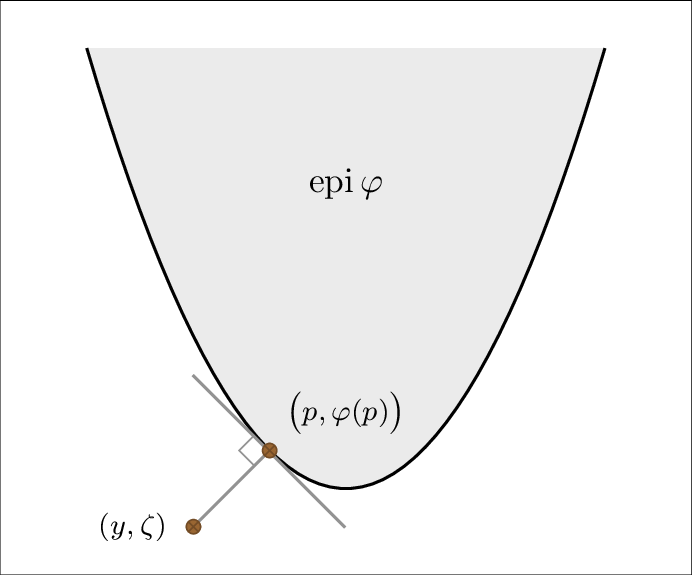
\includegraphics[width=0.45\linewidth]{epigraph}
			\caption{Эпиграф. \small{\href{https://www.researchgate.net/figure/Projection-onto-the-epigraph-of-a-function-ph-G-0-R_fig1_270905703}{Источник - ссылка}.} }
			\label{fig:epigraph}
		\end{figure}
		%
		Надграфик выпуклой функции является выпуклым. Касательная к функции является опорной гиперплоскостью к ее надграфику.}
		
	\end{flushleft}
\end{frame}

\begin{frame}{Выпуклые функции — примеры}
	\begin{flushleft}
		
		Вот некоторые выпуклые функции одной переменной:
		
		\begin{itemize}
			\item $f(x) = 1$
			\item $f(x) = x$; $f(x) = x + 1$, $f(x) = 6x + 3$
			\item $f(x) = x^2$; $f(x) = (x - 5)^2$; $f(x) = (x + 1)^2 - 10$
			\item $f(x) = x^3$, если $x > 0$
		\end{itemize}
		
		\bigskip
		
		Вот некоторые выпуклые функции многих переменных:
		
		\begin{itemize}
			\item $f(\mathbf{x}) = \mathbf{A}\mathbf{x} + \mathbf{b}$
			\item $f(\mathbf{x}) = \mathbf{x}^\top \mathbf{H}\mathbf{x}$, $\mathbf{H} \succ 0$
			\item $f(\mathbf{x}) = \text{max}(x_1, \ ... \ x_n) $
			\item $f(\mathbf{x}) = \text{log}(e^{x_1}+ ... +e^{x_n}) $
			\item $f(x, y) = \frac{x^2}{y}$, для $y > 0$
		\end{itemize}
		
	\end{flushleft}
\end{frame}

\begin{frame}{Выпуклое программирование}
	\begin{flushleft}
		
		\begin{block}{Определение 3}
			Если область определения задачи оптимизации является выпуклой, а целевая функция является выпуклой, то такая задача называется \emph{задачей выпуклой оптимизации}.
		\end{block}
		
		\bigskip
		
		Существует несколько важных свойств задач выпуклой оптимизации (с нашими дополнительными предположениями):
		
		\begin{itemize}
			\item Если область непуста, решение существует.
			\item Задача не имеет локальных минимумов. Мы можем найти путь из любой точки к решению, вдоль которого целевая функция не будет возрастать.
		\end{itemize}
		
	\end{flushleft}
\end{frame}



\begin{frame}{Пример — управление силой}
	\begin{flushleft}
		
		Рассмотрим манипулятор робота; сила на его концевом эффекторе связана с моментами в сочленениях уравнением $\bo{f} = \bo{J} \tau$. Найти такие моменты в сочленениях, которые создают выходную силу, наиболее близкую к желаемому значению $\bo{f}_d$, при этом моменты по компонентам ограничены по величине значением $\tau_{max}$.
		
		\bigskip
		
		\textbf{Решение}:
		%
		\begin{equation}
			\begin{aligned}
				& \underset{\tau, \bo{f}}{\text{minimize}}
				& & (\bo{f}-\bo{f}_d)\T (\bo{f}-\bo{f}_d), \\
				& \text{subject to}
				& & \begin{cases}
					\bo{f} = \bo{J} \tau \\
					|\tau_i| \leq \tau_{max}, \ \forall i
				\end{cases}
			\end{aligned}
		\end{equation}
		%
		Перепишем целевую функцию следующим образом:
		%
		\begin{align}
			(\bo{f}-\bo{f}_d)\T (\bo{f}-\bo{f}_d) = \bo{f}\T \bo{f} - 2 \bo{f}\T\bo{f}_d + \bo{f}_d\T \bo{f}_d
		\end{align}
		
		Целевая функция является \textbf{выпуклой} (она квадратичная), а область определения является \textbf{выпуклой}.
		
	\end{flushleft}
\end{frame}

\begin{frame}{Пример — обратная кинематика}
	\begin{flushleft}
		
		Рассмотрим перевернутый маятник; положение его точки описывается как $x = \cos(\varphi)$, $y = \sin(\varphi)$. Найти такой угол $\varphi$, который помещает точку наиболее близко к желаемому положению $x_d, y_d$.
		
		\bigskip
		
		\textbf{Решение}:
		%
		\begin{equation}
			\begin{aligned}
				& \underset{\varphi}{\text{minimize}}
				& & (\cos(\varphi)-x_d)^2 +
				(\sin(\varphi)-y_d)^2
			\end{aligned}
		\end{equation}
		
		Целевая функция \textbf{не является выпуклой}. См. ее график:
		
		\begin{figure}
			\centering
			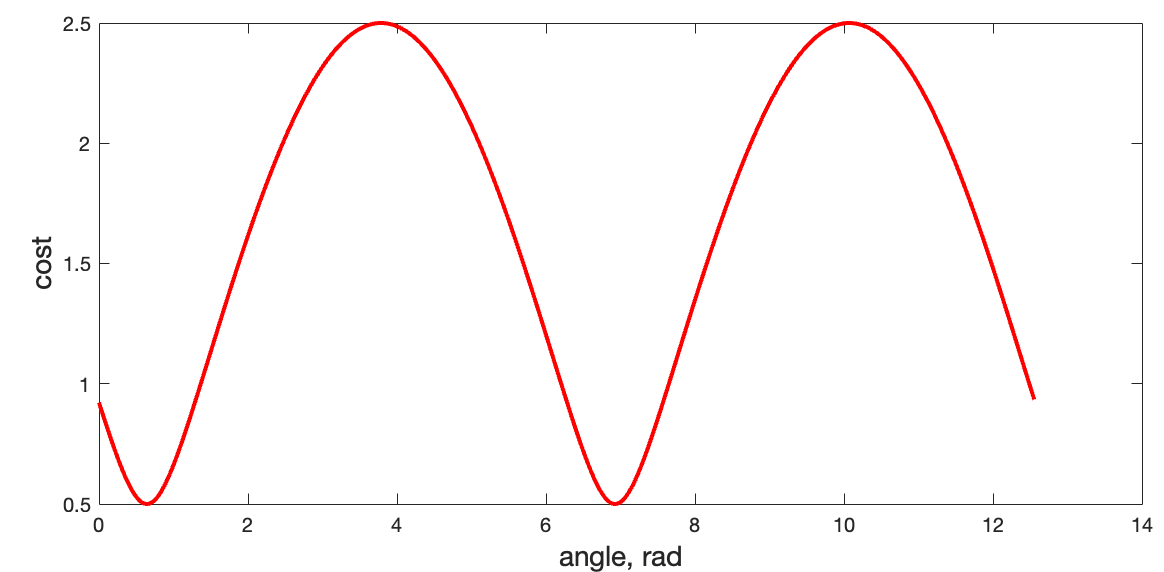
\includegraphics[height=0.4\textheight]{NonConvex}
		\end{figure}
		
	\end{flushleft}
\end{frame}


\begin{frame}{Литература}
	\begin{itemize}
		\item S. Boyd and L. Vandenberghe, \textit{Convex Optimization}, Cambridge University Press, 2004. \bref{https://web.stanford.edu/~boyd/cvxbook/bv\_cvxbook.pdf}{https://web.stanford.edu/~boyd/cvxbook/bv\_cvxbook.pdf}
	\end{itemize}
\end{frame}


\myqrframe

\begin{frame}{Приложение A. Типы областей определения}
	\begin{itemize}
		\item \textbf{Ограниченная}: переменные не могут становиться сколь угодно большими
		\item \textbf{Неограниченная}: переменные могут стремиться к бесконечности
		\item \textbf{Замкнутая}: содержит свою границу
		\item \textbf{Открытая}: не содержит своей границы
		\item \textbf{Компактная}: замкнутая и ограниченная
	\end{itemize}
\end{frame}

\end{document}
